\section{Odpowiedzi}

\subsection*{Gniazda klienckie TCP}
\begin{enumerate}[label=\textbf{3.\arabic*}]\setlength{\itemsep}{1em}
    \item    Aby przetestować poprawność swojego rozwiązania, możesz przeskanować swój własny komputer, żeby sprawdzić, czy skanowanie da taki sam wynik, jak Twój program. Do tego celu możesz wykorzystać np. narzędzie \texttt{nmap}. Zainstaluj \texttt{nmap}: \texttt{sudo apt install nmap}, a następnie wydaj polecenie: \texttt{nmap -p 22 localhost} (lub \texttt{nmap -p 22 127.0.0.1}) aby sprawdzić, czy port 22 jest otwarty na Twoim komputerze. Porównaj wynik z działaniem Twojego programu dla tego samego portu.  

\begin{figure}[h]
\caption{Wynik działania programu \texttt{nmap} dla lokalnej maszyny i portu \texttt{22}}
\centering
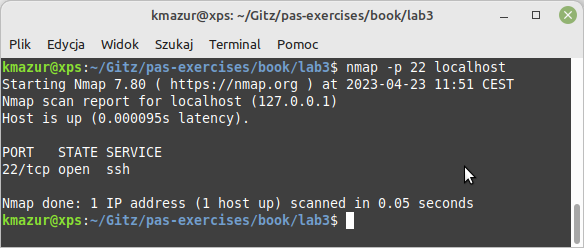
\includegraphics[scale=0.6]{./images/answers/ex3.1.png}
\end{figure}   
% #####################################################################################################

\item Możesz przetestować program używając swojego lokalnego adresu IPv6: \texttt{::1} lub \texttt{ip6-localhost} lub \\ \texttt{0000:0000:0000:0000:0000:0000:0000:0001}. 

\begin{figure}[h]
\caption{Wynik działania programu \texttt{nmap} dla lokalnej maszyny i portu \texttt{22}}
\centering
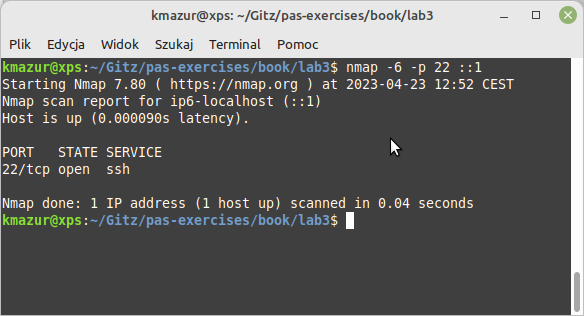
\includegraphics[scale=0.6]{./images/answers/ex3.2-nmap.png}
\end{figure}   
% #####################################################################################################

\newpage
\item Aby przetestować poprawność swojego rozwiązania, możesz przeskanować swój własny komputer, żeby sprawdzić, czy skanowanie da taki sam wynik, jak Twój program. Do tego celu możesz wykorzystać np. narzędzie \texttt{nmap}. Zainstaluj \texttt{nmap}: \texttt{sudo apt install nmap}, a następnie wydaj polecenie: \texttt{nmap -p1-65535 localhost} (lub \texttt{nmap -p1-65535 127.0.0.1}) aby sprawdzić, jakie porty są otwarte na Twoim komputerze. Porównaj wynik z działaniem Twojego programu dla tego samego portu.  

\begin{figure}[h]
\caption{Wynik działania programu \texttt{nmap} dla lokalnej maszyny i wszystkich jej portów}
\centering
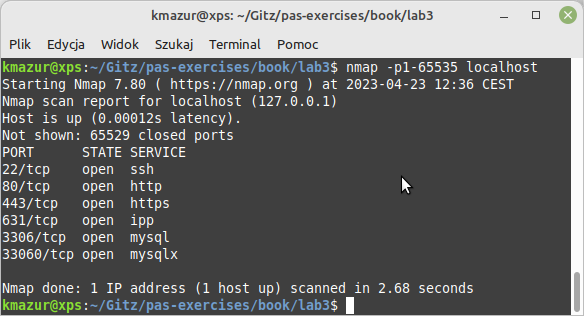
\includegraphics[scale=0.6]{./images/answers/ex3.3-nmap.png}
\end{figure}   
% #####################################################################################################

\item Aby przetestować poprawność swojego rozwiązania, możesz przeskanować swój własny komputer, żeby sprawdzić, czy skanowanie da taki sam wynik, jak Twój program. Do tego celu możesz wykorzystać np. narzędzie \texttt{nmap}. Zainstaluj \texttt{nmap}: \texttt{sudo apt install nmap}, a następnie wydaj polecenie: \texttt{nmap -6 -p1-65535 ip6-localhost} (lub \texttt{nmap -6 -p1-65535 ::1}) aby sprawdzić, jakie porty są otwarte na Twoim komputerze. Porównaj wynik z działaniem Twojego programu dla tego samego portu.  

\begin{figure}[h]
\caption{Wynik działania programu \texttt{nmap} dla lokalnej maszyny i wszystkich jej portów}
\centering
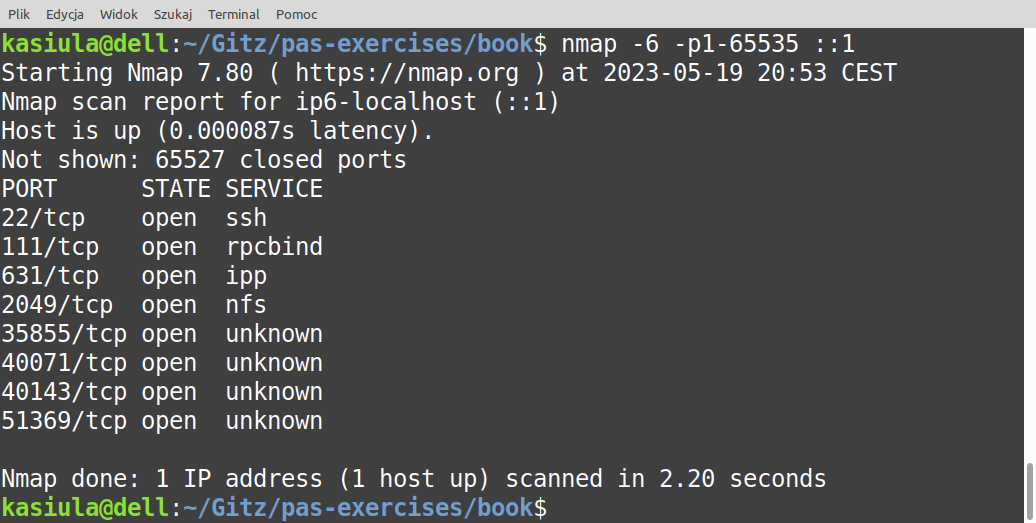
\includegraphics[scale=0.35]{./images/answers/ex3.4-nmap.png}
\end{figure}   
% #####################################################################################################

\item Aby przetestować poprawność swojego rozwiązania, możesz skorzystać z gotowego serwera, do którego może połączyć się Twój klient, aby pobrać aktualną datę i czas. Aby uruchomić serwer, zainstaluj \href{https://www.docker.com/}{Dockera}, a następnie w konsoli wydaj polecenia:

\begin{itemize}
\item Pobierz obraz serwera:\\ \texttt{docker pull mazurkatarzyna/pas-book-p1-ch3-ex5-server:latest}

\item Uruchom serwer za pomocą Dockera:\\ \texttt{docker run -dp 3005:3005 mazurkatarzyna/pas-book-p1-ch3-ex5-server}
\end{itemize}

\noindent Tak uruchomiony serwer działa na Twoim komputerze, jego adres IPv4 to \texttt{127.0.0.1} (\texttt{localhost}), numer portu to 3005.
% #####################################################################################################

\item Aby przetestować poprawność swojego rozwiązania, możesz skorzystać z gotowego serwera, do którego może połączyć się Twój klient, aby pobrać aktualną datę i czas. Aby uruchomić serwer, zainstaluj \href{https://www.docker.com/}{Dockera}, a następnie w konsoli wydaj polecenia:

\begin{itemize}
\item Pobierz obraz serwera:\\ \texttt{docker pull mazurkatarzyna/pas-book-p1-ch3-ex6-server:latest}

\item Uruchom serwer za pomocą Dockera:\\ \texttt{docker run -dp 3006:3006 mazurkatarzyna/pas-book-p1-ch3-ex6-server}
\end{itemize}

\noindent Tak uruchomiony serwer działa na Twoim komputerze, jego adres IPv6 to \texttt{::1} (\texttt{localhost}), numer portu to 3006.
% #####################################################################################################
\item Aby przetestować poprawność swojego rozwiązania, możesz skorzystać z gotowego serwera, do którego może połączyć się Twój klient, aby wysłać wiadomość. Aby uruchomić serwer, zainstaluj \href{https://www.docker.com/}{Dockera}, a następnie w konsoli wydaj polecenia:

\begin{itemize}
\item Pobierz obraz serwera:\\ \texttt{docker pull mazurkatarzyna/pas-book-p1-ch3-ex7-server:latest}

\item Uruchom serwer za pomocą Dockera:\\ \texttt{docker run -dp 3007:3007 mazurkatarzyna/pas-book-p1-ch3-ex7-server}
\end{itemize}

\noindent Tak uruchomiony serwer działa na Twoim komputerze, jego adres IPv4 to \texttt{127.0.0.1} (\texttt{localhost}), numer portu to 3007.
%#####################################################################################################

\item Aby przetestować poprawność swojego rozwiązania, możesz skorzystać z gotowego serwera, do którego może połączyć się Twój klient, aby wysłać wiadomość. Aby uruchomić serwer, zainstaluj \href{https://www.docker.com/}{Dockera}, a następnie w konsoli wydaj polecenia:

\begin{itemize}
\item Pobierz obraz serwera:\\ \texttt{docker pull mazurkatarzyna/pas-book-p1-ch3-ex8-server:latest}

\item Uruchom serwer za pomocą Dockera:\\ \texttt{docker run -dp 3008:3008 mazurkatarzyna/pas-book-p1-ch3-ex8-server}
\end{itemize}

\noindent Tak uruchomiony serwer działa na Twoim komputerze, jego adres IPv6 to \texttt{::1} (\texttt{localhost}), numer portu to 3008.
%#####################################################################################################
\item Aby przetestować poprawność swojego rozwiązania, możesz skorzystać z gotowego serwera, do którego może połączyć się Twój klient, aby wysłać wiadomość. Aby uruchomić serwer, zainstaluj \href{https://www.docker.com/}{Dockera}, a następnie w konsoli wydaj polecenia:

\begin{itemize}
\item Pobierz obraz serwera:\\ \texttt{docker pull mazurkatarzyna/pas-book-p1-ch3-ex9-server:latest}

\item Uruchom serwer za pomocą Dockera:\\ \texttt{docker run -dp 3009:3009 mazurkatarzyna/pas-book-p1-ch3-ex9-server}
\end{itemize}

\noindent Tak uruchomiony serwer działa na Twoim komputerze, jego adres IPv4 to \texttt{127.0.0.1} (\texttt{localhost}), numer portu to 3009.
%#####################################################################################################
\item Aby przetestować poprawność swojego rozwiązania, możesz skorzystać z gotowego serwera, do którego może połączyć się Twój klient, aby wysłać wiadomość. Aby uruchomić serwer, zainstaluj \href{https://www.docker.com/}{Dockera}, a następnie w konsoli wydaj polecenia:

\begin{itemize}
\item Pobierz obraz serwera:\\ \texttt{docker pull mazurkatarzyna/pas-book-p1-ch3-ex10-server:latest}

\item Uruchom serwer za pomocą Dockera:\\ \texttt{docker run -dp 3010:3010 mazurkatarzyna/pas-book-p1-ch3-ex10-server}
\end{itemize}

\noindent Tak uruchomiony serwer działa na Twoim komputerze, jego adres IPv6 to \texttt{::1} (\texttt{localhost}), numer portu to 3010.
%#####################################################################################################
 \item    Aby przetestować poprawność swojego rozwiązania, możesz przeskanować swój własny komputer, żeby sprawdzić, czy skanowanie da taki sam wynik, jak Twój program. Do tego celu możesz wykorzystać np. narzędzie \texttt{nmap} z parametrem \texttt{-{}-}\texttt{script=banner}. Zainstaluj \texttt{nmap}: \texttt{sudo apt install nmap}, a następnie wydaj polecenie: \texttt{nmap -p 22} \texttt{-{}-}\texttt{script=banner} \texttt{localhost} (lub \texttt{nmap -p 22} \texttt{-{}-}\texttt{script=banner} \texttt{127.0.0.1}) aby sprawdzić, czy port 22 jest otwarty na Twoim komputerze, i jaka usługa jest uruchomiona na tym porcie. Porównaj wynik z działaniem Twojego programu dla tego samego portu.  

\begin{figure}[h]
\caption{Wynik działania programu \texttt{nmap} dla lokalnej maszyny i portu \texttt{22}}
\centering
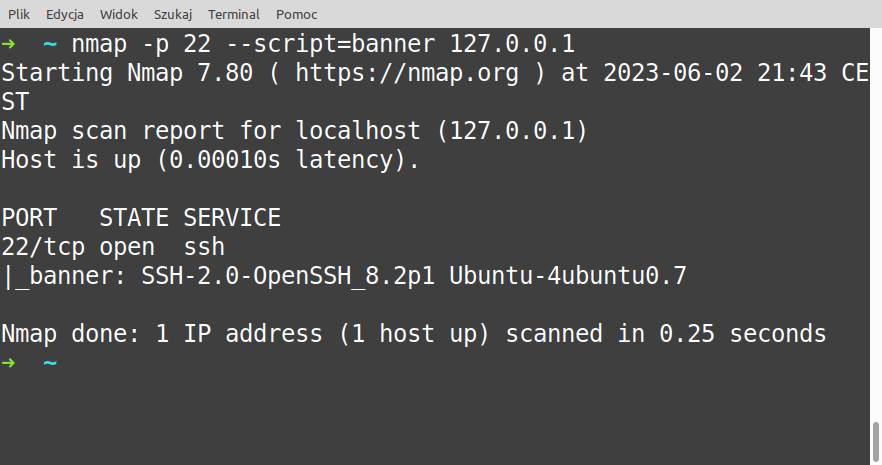
\includegraphics[scale=0.3]{./images/answers/ex3.11.png}
\end{figure}   
%#####################################################################################################
 \item    Aby przetestować poprawność swojego rozwiązania, możesz przeskanować swój własny komputer, żeby sprawdzić, czy skanowanie da taki sam wynik, jak Twój program. Do tego celu możesz wykorzystać np. narzędzie \texttt{nmap} z parametrem \texttt{-{}-}\texttt{script=banner}. Zainstaluj \texttt{nmap}: \texttt{sudo apt install nmap}, a następnie wydaj polecenie: \texttt{nmap -p 22 -6} \texttt{-{}-}\texttt{script=banner} \texttt{ip6-localhost} (lub \texttt{nmap -p 22 -6} \texttt{-{}-}\texttt{script=banner} \texttt{::1}) aby sprawdzić, czy port 22 jest otwarty na Twoim komputerze, i jaka usługa jest uruchomiona na tym porcie. Porównaj wynik z działaniem Twojego programu dla tego samego portu.  

\begin{figure}[h]
\caption{Wynik działania programu \texttt{nmap} dla lokalnej maszyny i portu \texttt{22}}
\centering
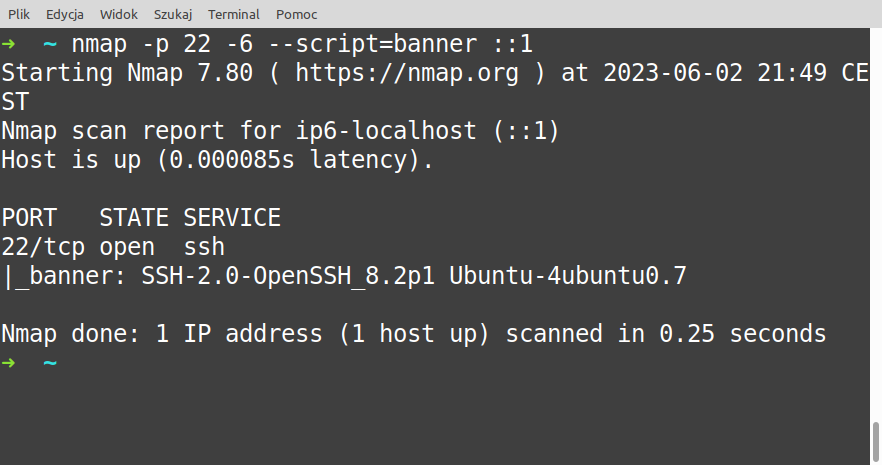
\includegraphics[scale=0.3]{./images/answers/ex3.12.png}
\end{figure}  

\end{enumerate}
%#####################################################################################################
\newpage
\subsection*{Protokoły pocztowe - protokół SMTP}
\begin{enumerate}[label=\textbf{6.\arabic*}]\setlength{\itemsep}{1em}
\item \label{answ61} Do wykonania zadania możesz użyć:
\begin{itemize}
	\item Klienta \texttt{telnet}, jeśli serwer nie wymaga szyfrowania, polecenie do nawiązania połączenia z serwerem: \texttt{telnet server\_ip port}
	\item Klienta \texttt{OpenSSL}, o nazwie \texttt{s\_client} jeśli serwer wymaga szyfrowania, polecenie do nawiązania połączenia z serwerem: \texttt{openssl s\_client -crlf -connect server\_ip:port}
\end{itemize}
\noindent Jako serwera SMTP możesz użyć:
\begin{itemize}
 \item \texttt{iRedMail}, który dostępny jest jako \href{https://hub.docker.com/r/iredmail/mariadb}{kontener Dockerowy}, 
 \item Serwera pocztowego udostępnianego np. przez \texttt{interia.pl}, gdzie \texttt{poczta.interia.pl} jest adresem serwera SMTP, \texttt{465} jest numerem portu, na którym działa serwer. Potrzebujesz również konta na serwerze.
 \end{itemize}
 \noindent Poniżej przykład połączenia z serwerem \texttt{poczta.interia.pl}:
 \begin{figure}[h]
\centering
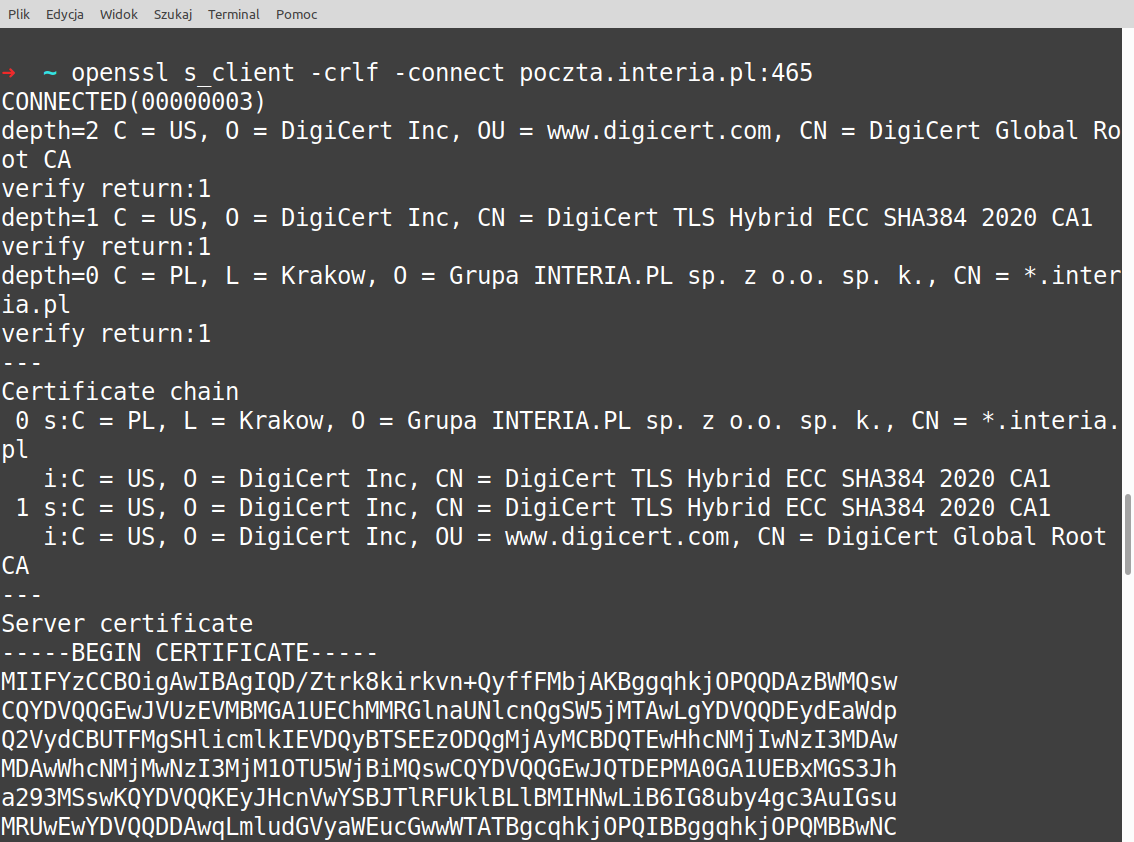
\includegraphics[scale=0.25]{./images/answers/smtp1.png}
\end{figure}  
 \begin{figure}[h]
\centering
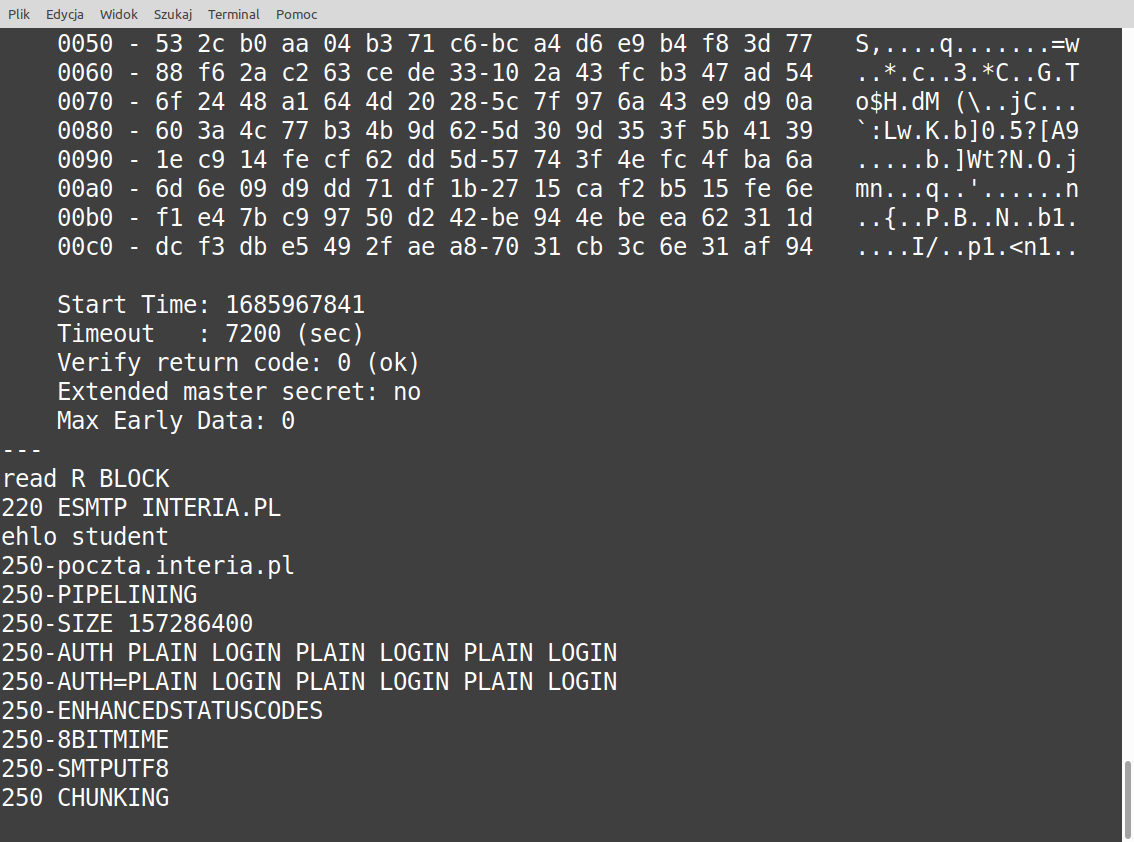
\includegraphics[scale=0.25]{./images/answers/smtp2.png}
\end{figure} 

\newpage 
\noindent Na niebiesko zaznaczono polecenia / komendy, których musisz użyć. Kolorem czarnym oznaczono odpowiedzi serwera:\\ \mbox{}
\scriptsize
\begin{alltt}
\textcolor{blue}{openssl s_client -crlf -connect poczta.interia.pl:465}
CONNECTED(00000003)
depth=2 C = US, O = DigiCert Inc, OU = www.digicert.com, CN = DigiCert Global Root CA
verify return:1
depth=1 C = US, O = DigiCert Inc, CN = DigiCert TLS Hybrid ECC SHA384 2020 CA1
verify return:1
depth=0 C = PL, L = Krakow, O = Grupa INTERIA.PL sp. z o.o. sp. k., CN = *.interia.pl
verify return:1
---
Certificate chain
 0 s:C = PL, L = Krakow, O = Grupa INTERIA.PL sp. z o.o. sp. k., CN = *.interia.pl
   i:C = US, O = DigiCert Inc, CN = DigiCert TLS Hybrid ECC SHA384 2020 CA1
 1 s:C = US, O = DigiCert Inc, CN = DigiCert TLS Hybrid ECC SHA384 2020 CA1
   i:C = US, O = DigiCert Inc, OU = www.digicert.com, CN = DigiCert Global Root CA
---
Server certificate
-----BEGIN CERTIFICATE-----
MIIFYzCCBOigAwIBAgIQD/Ztrk8kirkvn+QyffFMbjAKBggqhkjOPQQDAzBWMQsw
CQYDVQQGEwJVUzEVMBMGA1UEChMMRGlnaUNlcnQgSW5jMTAwLgYDVQQDEydEaWdp
Q2VydCBUTFMgSHlicmlkIEVDQyBTSEEzODQgMjAyMCBDQTEwHhcNMjIwNzI3MDAw
MDAwWhcNMjMwNzI3MjM1OTU5WjBiMQswCQYDVQQGEwJQTDEPMA0GA1UEBxMGS3Jh
a293MSswKQYDVQQKEyJHcnVwYSBJTlRFUklBLlBMIHNwLiB6IG8uby4gc3AuIGsu
MRUwEwYDVQQDDAwqLmludGVyaWEucGwwWTATBgcqhkjOPQIBBggqhkjOPQMBBwNC
AATj14S/K9d1aInT0/N6wXhyj7/0YxfJlR7jOxE8C5JiUZpaip8/DDL7syoNB3xS
LtJIpG1Ygqy9kRHr8wfIVOCzo4IDijCCA4YwHwYDVR0jBBgwFoAUCrwIKReMpTlt
eg7OM8cus+37w3owHQYDVR0OBBYEFEzd3VGbvBiH2K8Z1aE6Py9C0HHNMCMGA1Ud
EQQcMBqCDCouaW50ZXJpYS5wbIIKaW50ZXJpYS5wbDAOBgNVHQ8BAf8EBAMCB4Aw
HQYDVR0lBBYwFAYIKwYBBQUHAwEGCCsGAQUFBwMCMIGbBgNVHR8EgZMwgZAwRqBE
oEKGQGh0dHA6Ly9jcmwzLmRpZ2ljZXJ0LmNvbS9EaWdpQ2VydFRMU0h5YnJpZEVD
Q1NIQTM4NDIwMjBDQTEtMS5jcmwwRqBEoEKGQGh0dHA6Ly9jcmw0LmRpZ2ljZXJ0
LmNvbS9EaWdpQ2VydFRMU0h5YnJpZEVDQ1NIQTM4NDIwMjBDQTEtMS5jcmwwPgYD
VR0gBDcwNTAzBgZngQwBAgIwKTAnBggrBgEFBQcCARYbaHR0cDovL3d3dy5kaWdp
Y2VydC5jb20vQ1BTMIGFBggrBgEFBQcBAQR5MHcwJAYIKwYBBQUHMAGGGGh0dHA6
Ly9vY3NwLmRpZ2ljZXJ0LmNvbTBPBggrBgEFBQcwAoZDaHR0cDovL2NhY2VydHMu
ZGlnaWNlcnQuY29tL0RpZ2lDZXJ0VExTSHlicmlkRUNDU0hBMzg0MjAyMENBMS0x
LmNydDAJBgNVHRMEAjAAMIIBfQYKKwYBBAHWeQIEAgSCAW0EggFpAWcAdQCt9776
fP8QyIudPZwePhhqtGcpXc+xDCTKhYY069yCigAAAYJBhgsMAAAEAwBGMEQCIELl
g7IxBfCpgigx/rDU7kUvWaYWvMxf0tRkTL2UHbSVAiBIGwYMqfuFuoThbrny0stk
O4hwJoak4J69MvZ+HasnAQB2ADXPGRu/sWxXvw+tTG1Cy7u2JyAmUeo/4SrvqAPD
O9ZMAAABgkGGCtYAAAQDAEcwRQIhAPFjNAwBAB5v0G0Qw0uaDWMF7n3n/7s2t7gZ
Nlhy6Z8sAiBcLcCvAP/llzyfk/5olh01c85cWB6+HD3if6BUoUNMlgB2ALNzdwfh
hFD4Y4bWBancEQlKeS2xZwwLh9zwAw55NqWaAAABgkGGCwEAAAQDAEcwRQIgSsPk
X+yBkecqv0CuIXmWg9V2e/s4LYyYvsuIJU7ksxgCIQDkrabch4m6Sg9U6AaqeW8M
vPtFrIjAzwSymXt2lNyKTDAKBggqhkjOPQQDAwNpADBmAjEAv+cUUU3e9sdRaOFs
ntdpEVKb4S71HWCsVRZcS2MGIMOZRJ5LVEhhXHKl+EIaJ257AjEA8rSvrwL4MIRz
fCA70evopfs2fJcQVU4TLEbSFBwkAdh0LlHAnXH+NELH1ttjQtfh
-----END CERTIFICATE-----
subject=C = PL, L = Krakow, O = Grupa INTERIA.PL sp. z o.o. sp. k., CN = *.interia.pl

issuer=C = US, O = DigiCert Inc, CN = DigiCert TLS Hybrid ECC SHA384 2020 CA1

---
No client certificate CA names sent
Peer signing digest: SHA256
Peer signature type: ECDSA
Server Temp Key: X25519, 253 bits
---
SSL handshake has read 2811 bytes and written 389 bytes
Verification: OK
---
New, TLSv1.3, Cipher is TLS_AES_256_GCM_SHA384
Server public key is 256 bit
Secure Renegotiation IS NOT supported
Compression: NONE
Expansion: NONE
No ALPN negotiated
Early data was not sent
Verify return code: 0 (ok)
---
---
Post-Handshake New Session Ticket arrived:
SSL-Session:
    Protocol  : TLSv1.3
    Cipher    : TLS_AES_256_GCM_SHA384
    Session-ID: FA72D8E642670674F87A2BF7DE7D8716408D48DB0AF3F21F374FC989B6944C41
    Session-ID-ctx: 
    Resumption PSK: 
    328002BF74A3AC45B3D49DB69A6CEEBB80D17CFE1DE2BD71184A508001BABB1DC480C737B60DA4B6C43C40C1068039A2
    PSK identity: None
    PSK identity hint: None
    SRP username: None
    TLS session ticket lifetime hint: 7200 (seconds)
    TLS session ticket:
    0000 - d6 18 a0 85 49 b4 4b 4d-46 6d 71 b6 5f 38 ce 17   ....I.KMFmq._8..
    0010 - be e4 36 99 4d 17 4c ce-8b 13 6f 61 0b 3d e6 17   ..6.M.L...oa.=..
    0020 - 51 53 d6 d3 bf fc da 87-0f 38 eb 9c f0 fd 0e 5d   QS.......8.....]
    0030 - c0 9d 2f 95 e4 b3 78 24-98 b8 cd b4 83 50 08 43   ../...x\$.....P.C
    0040 - 1b e8 2b eb cd ee 3d 20-ef d6 4e 89 9d a6 21 92   ..+...= ..N...!.
    0050 - a7 0e 9b 04 e1 1e 9f 36-3f 6d 7b a5 a9 37 7d af   .......6?m\{..7\}.
    0060 - b4 3a 52 dc 68 7a 35 3b-89 74 89 ea ae 34 ba 46   .:R.hz5;.t...4.F
    0070 - fb e6 c6 da c3 f9 c1 89-f4 1e 89 28 50 32 12 74   ...........(P2.t
    0080 - 07 55 d0 7d 70 2f 1d e0-02 ca 6a e7 41 25 8f 53   .U.\}p/....j.A\%.S
    0090 - 5e 67 1d 25 f5 9f ab f9-e5 ce 0d 4d 05 78 46 4f   ^g.\%.......M.xFO
    00a0 - 11 d4 bb 3b 84 d2 26 71-28 3d 0b 13 a9 aa 85 95   ...;..&q(=......
    00b0 - 8d 77 c9 d0 be e5 d3 38-51 b1 1b f2 8b 9f 7e 8c   .w.....8Q.....~.
    00c0 - bb e9 5a f4 f9 71 40 3d-a1 1c 5b fe 35 c3 74 bf   ..Z..q@=..[.5.t.

    Start Time: 1685969504
    Timeout   : 7200 (sec)
    Verify return code: 0 (ok)
    Extended master secret: no
    Max Early Data: 0
---
read R BLOCK
220 ESMTP INTERIA.PL
\textcolor{blue}{ehlo student}
250-poczta.interia.pl
250-PIPELINING
250-SIZE 157286400
250-AUTH PLAIN LOGIN PLAIN LOGIN PLAIN LOGIN
250-AUTH=PLAIN LOGIN PLAIN LOGIN PLAIN LOGIN
250-ENHANCEDSTATUSCODES
250-8BITMIME
250-SMTPUTF8
250 CHUNKING
\textcolor{blue}{auth login}
334 VXNlcm5hbWU6
\textcolor{blue}{a29jaGFtLnVtY3NAaW50ZXJpYS5wbA==}
334 UGFzc3dvcmQ6
\textcolor{blue}{a29jaGFtLnVtY3MyMDIz}
235 2.7.0 Authentication successful
\textcolor{blue}{mail from: <kocham.umcs@interia.pl>}
250 2.1.0 Ok
\textcolor{blue}{rcpt to: <pas.umcs@poczta.fm>}
250 2.1.5 Ok
\textcolor{blue}{data}
354 End data with <CR><LF>.<CR><LF>
\textcolor{blue}{to: <pas.umcs@poczta.fm>}
\textcolor{blue}{from: <kocham.umcs@interia.pl>}    
\textcolor{blue}{subject: test email}

\textcolor{blue}{Hello!}

\textcolor{blue}{.}
250 OK. ID: 1054c830c3886b54
\textcolor{blue}{quit}
221 2.0.0 Bye
closed
\end{alltt}

\normalsize
\item Możesz skorzystać z jednego z serwerów SMTP zaproponowanego w rozwiązaniu do zadania \ref{answ61}. Jaka komenda protokołu SMTP pozwala na określenie odbiorcy wiadomości? 

\item Możesz skorzystać z jednego z serwerów SMTP zaproponowanego w rozwiązaniu do zadania \ref{answ61}. Jaka komenda protokołu SMTP pozwala na określenie nadawcy wiadomości? 

\item Możesz skorzystać z jednego z serwerów SMTP zaproponowanego w rozwiązaniu do zadania \ref{answ61}. Pamiętaj, że każda nowa linia ma znaczenie. Jeśli nie zachowasz odpowiedniej składni, serwer może ''nie zrozumieć'' wiadomości. Poniżej przykładowe rozwiązanie.  

\scriptsize
\begin{alltt}
\textcolor{blue}{openssl s_client -crlf -connect poczta.interia.pl:465}
CONNECTED(00000003)
depth=2 C = US, O = DigiCert Inc, OU = www.digicert.com, CN = DigiCert Global Root CA
verify return:1
depth=1 C = US, O = DigiCert Inc, CN = DigiCert TLS Hybrid ECC SHA384 2020 CA1
verify return:1
depth=0 C = PL, L = Krakow, O = Grupa INTERIA.PL sp. z o.o. sp. k., CN = *.interia.pl
verify return:1
---
Certificate chain
 0 s:C = PL, L = Krakow, O = Grupa INTERIA.PL sp. z o.o. sp. k., CN = *.interia.pl
   i:C = US, O = DigiCert Inc, CN = DigiCert TLS Hybrid ECC SHA384 2020 CA1
 1 s:C = US, O = DigiCert Inc, CN = DigiCert TLS Hybrid ECC SHA384 2020 CA1
   i:C = US, O = DigiCert Inc, OU = www.digicert.com, CN = DigiCert Global Root CA
---
Server certificate
-----BEGIN CERTIFICATE-----
MIIFYzCCBOigAwIBAgIQD/Ztrk8kirkvn+QyffFMbjAKBggqhkjOPQQDAzBWMQsw
CQYDVQQGEwJVUzEVMBMGA1UEChMMRGlnaUNlcnQgSW5jMTAwLgYDVQQDEydEaWdp
Q2VydCBUTFMgSHlicmlkIEVDQyBTSEEzODQgMjAyMCBDQTEwHhcNMjIwNzI3MDAw
MDAwWhcNMjMwNzI3MjM1OTU5WjBiMQswCQYDVQQGEwJQTDEPMA0GA1UEBxMGS3Jh
a293MSswKQYDVQQKEyJHcnVwYSBJTlRFUklBLlBMIHNwLiB6IG8uby4gc3AuIGsu
MRUwEwYDVQQDDAwqLmludGVyaWEucGwwWTATBgcqhkjOPQIBBggqhkjOPQMBBwNC
AATj14S/K9d1aInT0/N6wXhyj7/0YxfJlR7jOxE8C5JiUZpaip8/DDL7syoNB3xS
LtJIpG1Ygqy9kRHr8wfIVOCzo4IDijCCA4YwHwYDVR0jBBgwFoAUCrwIKReMpTlt
eg7OM8cus+37w3owHQYDVR0OBBYEFEzd3VGbvBiH2K8Z1aE6Py9C0HHNMCMGA1Ud
EQQcMBqCDCouaW50ZXJpYS5wbIIKaW50ZXJpYS5wbDAOBgNVHQ8BAf8EBAMCB4Aw
HQYDVR0lBBYwFAYIKwYBBQUHAwEGCCsGAQUFBwMCMIGbBgNVHR8EgZMwgZAwRqBE
oEKGQGh0dHA6Ly9jcmwzLmRpZ2ljZXJ0LmNvbS9EaWdpQ2VydFRMU0h5YnJpZEVD
Q1NIQTM4NDIwMjBDQTEtMS5jcmwwRqBEoEKGQGh0dHA6Ly9jcmw0LmRpZ2ljZXJ0
LmNvbS9EaWdpQ2VydFRMU0h5YnJpZEVDQ1NIQTM4NDIwMjBDQTEtMS5jcmwwPgYD
VR0gBDcwNTAzBgZngQwBAgIwKTAnBggrBgEFBQcCARYbaHR0cDovL3d3dy5kaWdp
Y2VydC5jb20vQ1BTMIGFBggrBgEFBQcBAQR5MHcwJAYIKwYBBQUHMAGGGGh0dHA6
Ly9vY3NwLmRpZ2ljZXJ0LmNvbTBPBggrBgEFBQcwAoZDaHR0cDovL2NhY2VydHMu
ZGlnaWNlcnQuY29tL0RpZ2lDZXJ0VExTSHlicmlkRUNDU0hBMzg0MjAyMENBMS0x
LmNydDAJBgNVHRMEAjAAMIIBfQYKKwYBBAHWeQIEAgSCAW0EggFpAWcAdQCt9776
fP8QyIudPZwePhhqtGcpXc+xDCTKhYY069yCigAAAYJBhgsMAAAEAwBGMEQCIELl
g7IxBfCpgigx/rDU7kUvWaYWvMxf0tRkTL2UHbSVAiBIGwYMqfuFuoThbrny0stk
O4hwJoak4J69MvZ+HasnAQB2ADXPGRu/sWxXvw+tTG1Cy7u2JyAmUeo/4SrvqAPD
O9ZMAAABgkGGCtYAAAQDAEcwRQIhAPFjNAwBAB5v0G0Qw0uaDWMF7n3n/7s2t7gZ
Nlhy6Z8sAiBcLcCvAP/llzyfk/5olh01c85cWB6+HD3if6BUoUNMlgB2ALNzdwfh
hFD4Y4bWBancEQlKeS2xZwwLh9zwAw55NqWaAAABgkGGCwEAAAQDAEcwRQIgSsPk
X+yBkecqv0CuIXmWg9V2e/s4LYyYvsuIJU7ksxgCIQDkrabch4m6Sg9U6AaqeW8M
vPtFrIjAzwSymXt2lNyKTDAKBggqhkjOPQQDAwNpADBmAjEAv+cUUU3e9sdRaOFs
ntdpEVKb4S71HWCsVRZcS2MGIMOZRJ5LVEhhXHKl+EIaJ257AjEA8rSvrwL4MIRz
fCA70evopfs2fJcQVU4TLEbSFBwkAdh0LlHAnXH+NELH1ttjQtfh
-----END CERTIFICATE-----
subject=C = PL, L = Krakow, O = Grupa INTERIA.PL sp. z o.o. sp. k., CN = *.interia.pl

issuer=C = US, O = DigiCert Inc, CN = DigiCert TLS Hybrid ECC SHA384 2020 CA1

---
No client certificate CA names sent
Peer signing digest: SHA256
Peer signature type: ECDSA
Server Temp Key: X25519, 253 bits
---
SSL handshake has read 2810 bytes and written 389 bytes
Verification: OK
---
New, TLSv1.3, Cipher is TLS_AES_256_GCM_SHA384
Server public key is 256 bit
Secure Renegotiation IS NOT supported
Compression: NONE
Expansion: NONE
No ALPN negotiated
Early data was not sent
Verify return code: 0 (ok)
---
---
Post-Handshake New Session Ticket arrived:
SSL-Session:
    Protocol  : TLSv1.3
    Cipher    : TLS_AES_256_GCM_SHA384
    Session-ID: F75D463B69633B1F1958D6CE033697EAC3AC78E1ABAA461599D03B4822ACCEE6
    Session-ID-ctx: 
    Resumption PSK: 74B14972C5CC86292F1A2869821072E8A55177841455905EE18CA32CC871922F62A95CCA9B68450180CCD5D937D57981
    PSK identity: None
    PSK identity hint: None
    SRP username: None
    TLS session ticket lifetime hint: 7200 (seconds)
    TLS session ticket:
    0000 - a9 09 45 e3 8a 1e 19 3c-8a f7 6c ae 0e 95 f1 62   ..E....<..l....b
    0010 - ac 28 8e 1c aa 29 02 42-86 75 c5 88 5e 2f f3 c6   .(...).B.u..^/..
    0020 - 44 87 f9 04 91 ce 7e 6c-1d 0f 18 9a be 7d 11 56   D.....~l.....\}.V
    0030 - 73 71 be 37 61 bd 3e 8c-64 d2 7f d4 3c 7b 90 ab   sq.7a.>.d...<\{..
    0040 - fd 63 f7 c6 dd d5 3b a6-d6 cf 08 35 d8 42 88 a8   .c....;....5.B..
    0050 - be 40 5b fa a9 a3 40 57-85 3d 5e 6c b6 d7 97 36   .@[...@W.=^l...6
    0060 - 4c 17 41 f1 d1 da e8 79-49 81 36 bc 95 5e 09 c4   L.A....yI.6..^..
    0070 - 88 78 16 99 b0 28 e5 12-30 aa 5f f9 35 ac 2a c8   .x...(..0._.5.*.
    0080 - 79 68 51 93 0d 5d 5c 50-1a 5a ed 84 7f ee c1 7a   yhQ..]\P.Z.....z
    0090 - 10 d9 50 81 4c 9c 7d 75-9b f5 33 d7 09 85 43 1c   ..P.L.\}u..3...C.
    00a0 - e0 54 ca e0 f9 bc 39 a3-55 c1 82 e2 82 96 a8 ef   .T....9.U.......
    00b0 - a3 99 6e 61 e7 a5 e0 7f-c8 e9 77 16 14 ad 08 81   ..na......w.....
    00c0 - dd 93 df 4f db 13 d5 d0-5d 74 7b 71 aa 12 26 a2   ...O....]t\{q..&.

    Start Time: 1685976897
    Timeout   : 7200 (sec)
    Verify return code: 0 (ok)
    Extended master secret: no
    Max Early Data: 0
---
read R BLOCK
220 ESMTP INTERIA.PL
\textcolor{blue}{ehlo student}
250-poczta.interia.pl
250-PIPELINING
250-SIZE 157286400
250-AUTH PLAIN LOGIN PLAIN LOGIN PLAIN LOGIN
250-AUTH=PLAIN LOGIN PLAIN LOGIN PLAIN LOGIN
250-ENHANCEDSTATUSCODES
250-8BITMIME
250-SMTPUTF8
250 CHUNKING
\textcolor{blue}{auth login}
334 VXNlcm5hbWU6
\textcolor{blue}{a29jaGFtLnVtY3NAaW50ZXJpYS5wbA==}
334 UGFzc3dvcmQ6
\textcolor{blue}{a29jaGFtLnVtY3MyMDIz}
235 2.7.0 Authentication successful
\textcolor{blue}{mail from: <kocham.umcs@interia.pl>}
250 2.1.0 Ok
\textcolor{blue}{rcpt to: <pas.umcs@poczta.fm>}
250 2.1.5 Ok
\textcolor{blue}{data}
354 End data with <CR><LF>.<CR><LF>
\textcolor{blue}{to: <pas.umcs@poczta.fm>}
\textcolor{blue}{from: <kocham.umcs@interia.pl>}
\textcolor{blue}{subject: test email}
\textcolor{blue}{MIME-Version: 1.0}
\textcolor{blue}{Content-Type: multipart/mixed; boundary=sep}

\textcolor{blue}{--sep}

\textcolor{blue}{To}
\textcolor{blue}{jest}
\textcolor{blue}{Tresc wiadomosci}
\textcolor{blue}{--sep}
\textcolor{blue}{Content-Type: text/x-log; name=text.log}
\textcolor{blue}{Content-Disposition: attachment; filename=text.log}
\textcolor{blue}{Content-Transfer-Encoding: base64}
\textcolor{blue}{SGVsbG8K}
\textcolor{blue}{--sep--}
\textcolor{blue}{.}
250 OK. ID: bb63e06c9c318562
\textcolor{blue}{quit}
221 2.0.0 Bye
closed
\end{alltt}
\normalsize

\noindent Po sprawdzeniu swojej skrzynki pocztowej, powinieneś zobaczyć wysłaną wiadomość wraz z załącznikiem: \\

 \begin{figure}[h]
\centering
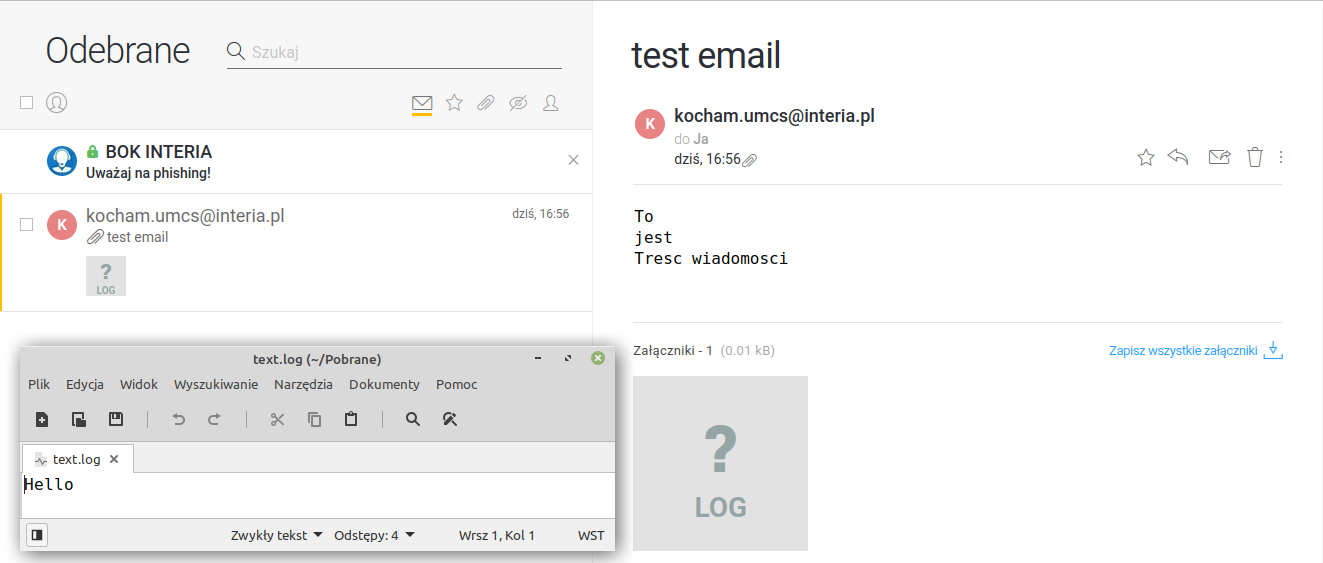
\includegraphics[scale=0.35]{./images/answers/email1.png}
\end{figure} 

\item Możesz skorzystać z jednego z serwerów SMTP zaproponowanego w rozwiązaniu do zadania \ref{answ61}. Pamiętaj, że każda nowa linia ma znaczenie. Jeśli nie zachowasz odpowiedniej składni, serwer może ''nie zrozumieć'' wiadomości. Poniżej przykładowe rozwiązanie.  

\scriptsize
\begin{verbatim}
telnet interia.pl 587
Trying 217.74.65.23...
Connected to interia.pl.
Escape character is '^]'.
220 ESMTP INTERIA.PL
HELO student
AUTH LOGIN
cGFzMjAxN0BpbnRlcmlhLnBs
UDRTSW5mMjAxNw==
MAIL FROM: <pas2017@interia.pl>
RCPT TO: <pas2017@interia.pl>
RCPT TO: <kasiula.mazur@gmail.com>
DATA

From: Nathaniel Borenstein <nsb@bellcore.com> 
To:  Ned Freed <ned@innosoft.com> 
Subject: Sample message 
MIME-Version: 1.0 
Content-Type: multipart/mixed; boundary=sep

--sep 

tresc wiadomosci
--sep
Content-Type: application/octet-stream; name=\"image.png\"
Content-Disposition: attachment; filename=\"image.png\"
Content-Transfer-Encoding: base64

/9j/4AAQSkZJRgABAQAAAQABAAD//gA7Q1JFQVRPUjogZ2QtanBlZyB2MS4wICh1
c2luZyBJSkcgSlBFRyB2NjIpLCBxdWFsaXR5ID0gODAK/9sAQwAGBAUGBQQGBgUG
BwcGCAoQCgoJCQoUDg8MEBcUGBgXFBYWGh0lHxobIxwWFiAsICMmJykqKRkfLTAt
KDAlKCko/9sAQwEHBwcKCAoTCgoTKBoWGigoKCgoKCgoKCgoKCgoKCgoKCgoKCgo
KCgoKCgoKCgoKCgoKCgoKCgoKCgoKCgoKCgo/8AAEQgGLgS9AwEiAAIRAQMRAf/E
...
--sep--
.
250 OK. ID: 1054c830c3886b54
QUIT
221 2.0.0 Bye
closed
\end{verbatim}
\normalsize

\newpage 
\item Możesz skorzystać z jednego z serwerów SMTP zaproponowanego w rozwiązaniu do zadania \ref{answ61}. Poniżej przykład nawiązania połączenia z serwerem (połączenie szyfrowane), i odebrania od serwera pierwszej wiadomości po połączeniu: \\  

\begin{figure}[h]
%\caption{Wynik działania programu \texttt{nmap} dla lokalnej maszyny i portu \texttt{22}}
\centering
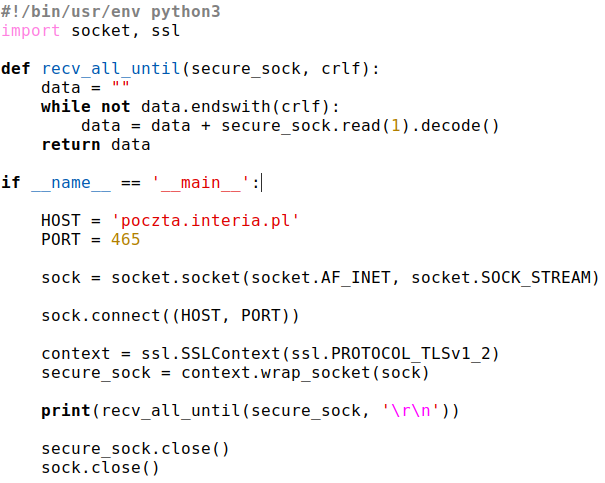
\includegraphics[scale=0.45]{./images/answers/smtp-py.png}
\end{figure}  

\item Możesz skorzystać z jednego z serwerów SMTP zaproponowanego w rozwiązaniu do zadania \ref{answ61}. 

\end{enumerate}

%#####################################################################################################
\newpage
\subsection*{Protokół HTTP}

\begin{enumerate}[label=\textbf{7.\arabic*}]\setlength{\itemsep}{1em}
\item Serwer możesz uruchomić za pomocą poniższych poleceń:

\begin{verbatim}
docker pull mazurkatarzyna/pas-book-p1-ch7-ex1:latest
docker run -dp 7001:80 mazurkatarzyna/pas-book-p1-ch7-ex1
\end{verbatim}

\noindent Działanie serwera możesz przetestować za pomocą przeglądarki. W swojej przeglądarce otwórz stronę: \url{http://127.0.0.1:7001/html}

% #################################################################################################################
\item Serwer możesz uruchomić za pomocą poniższych poleceń:

\begin{verbatim}
docker pull mazurkatarzyna/pas-book-p1-ch7-ex2:latest
docker run -dp 7002:80 mazurkatarzyna/pas-book-p1-ch7-ex2
\end{verbatim}

\noindent Działanie serwera możesz przetestować za pomocą przeglądarki. W swojej przeglądarce otwórz stronę: \url{http://127.0.0.1:7002/image/png}

% #################################################################################################################
\item Serwer możesz uruchomić za pomocą poniższych poleceń:

\begin{verbatim}
docker pull mazurkatarzyna/pas-book-p1-ch7-ex3:latest
docker run -dp 7003:80 mazurkatarzyna/pas-book-p1-ch7-ex3
\end{verbatim}

\noindent Działanie serwera możesz przetestować za pomocą przeglądarki. W swojej przeglądarce otwórz stronę: \url{http://127.0.0.1:7003/image.jpg}

% #################################################################################################################
\item Serwer możesz uruchomić za pomocą poniższych poleceń:

\begin{verbatim}
docker pull mazurkatarzyna/pas-book-p1-ch7-ex4:latest
docker run -dp 7004:80 mazurkatarzyna/pas-book-p1-ch7-ex4
\end{verbatim}

\noindent Działanie serwera możesz przetestować za pomocą przeglądarki. W swojej przeglądarce otwórz stronę: \url{http://127.0.0.1:7004/post}
% #################################################################################################################
\item Serwer możesz uruchomić za pomocą poniższych poleceń:

\begin{verbatim}
docker pull mazurkatarzyna/pas-book-p1-ch7-ex5:latest
docker run -dp 7005:80 mazurkatarzyna/pas-book-p1-ch7-ex5
\end{verbatim}

\noindent Działanie serwera możesz przetestować za pomocą przeglądarki. W swojej przeglądarce otwórz stronę: \url{http://127.0.0.1:7005}. Działający serwer powinien wyświetlać obrazek. W przypadku ataku DDoS, serwer będzie miał trudności w załadowaniu strony. Aby przetestować, czy Twój atak DDoS typu Slowloris jest skuteczny, możesz wykorzystać gotowe narzędzia, np. \url{https://github.com/gkbrk/slowloris} i zaatakować serwer.

% #################################################################################################################

\item 

% #################################################################################################################
\item Serwer możesz uruchomić za pomocą poniższych poleceń:

\begin{verbatim}
docker pull mazurkatarzyna/pas-book-p1-ch7-ex3:latest
docker run -dp 7003:80 mazurkatarzyna/pas-book-p1-ch7-ex3
\end{verbatim}

\noindent Działanie serwera możesz przetestować za pomocą przeglądarki. W swojej przeglądarce otwórz stronę: \url{http://127.0.0.1:7003/image.jpg}


\end{enumerate}
